% The inflaton rolling down its potential, and the fluctuations it leaves behind.
% After figures/chap2/inflation_potential.tex in the thesis, redrawn for a slide.
% Compile: pdflatex inflation_potential.tex && pdftocairo -svg inflation_potential.pdf inflation_potential.svg
\documentclass[tikz,border=4pt]{standalone}
\usepackage{tikz}
\usepackage{xcolor}
\usepackage{amsmath}
\usepackage[T1]{fontenc}
\usetikzlibrary{decorations.pathmorphing,arrows.meta,calc,patterns}

\definecolor{ink}{HTML}{2E2E2E}
\definecolor{greytx}{HTML}{6E6E6E}
\definecolor{curve}{HTML}{3B6FB6}
\definecolor{kw}{HTML}{C2560A}
\definecolor{kwtwo}{HTML}{521463}

\begin{document}
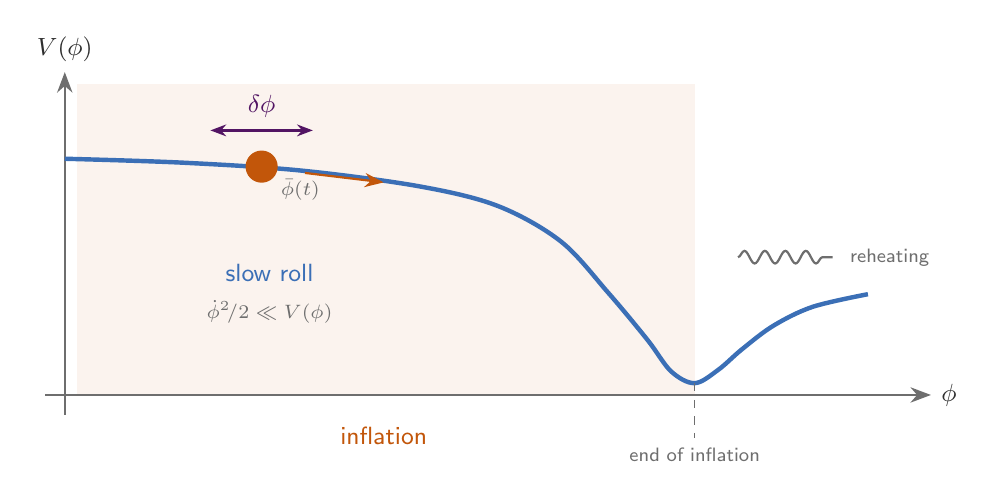
\begin{tikzpicture}[font=\sffamily\small,
    axis/.style={-{Stealth[length=2.6mm]},thick,greytx}]

  % Shaded stretch over which inflation happens.
  \fill[kw,opacity=0.07] (0.15,0) rectangle (8.0,3.95);

  \draw[axis] (-0.25,0) -- (11.0,0) node[right,ink]{$\phi$};
  \draw[axis] (0,-0.25) -- (0,4.1) node[above,ink]{$V(\phi)$};

  \draw[line width=1.6pt,curve]
    plot[smooth,tension=0.55] coordinates {
      (0.0,3.00) (1.5,2.95) (3.0,2.85) (4.5,2.65) (5.5,2.40)
      (6.3,1.95) (6.9,1.30) (7.4,0.70) (7.7,0.30) (8.0,0.15)
      (8.3,0.32) (8.6,0.58) (9.0,0.88) (9.5,1.12) (10.2,1.28)};

  % The inflaton, and the quantum fluctuation about its mean position.
  \draw[{Stealth[length=2.0mm]}-{Stealth[length=2.0mm]},kwtwo,thick]
        (1.85,3.36) -- (3.15,3.36);
  \node[kwtwo,above] at (2.5,3.40) {$\delta\phi$};
  \fill[kw] (2.5,2.90) circle (0.19);
  \draw[kw,thick] (2.5,2.90) circle (0.19);
  \node[greytx,below right,font=\sffamily\scriptsize] at (2.62,2.86) {$\bar\phi(t)$};
  \draw[-{Stealth[length=2.4mm]},kw,thick] (3.05,2.82) -- (4.05,2.70);

  \node[curve,font=\sffamily\small] at (2.6,1.55) {slow roll};
  \node[curve,font=\sffamily\scriptsize,text=greytx] at (2.6,1.05)
       {$\dot\phi^{2}\!/2 \ll V(\phi)$};

  \draw[greytx,dashed,thin] (8.0,0.15) -- (8.0,-0.55);
  \node[greytx,font=\sffamily\scriptsize,below] at (8.0,-0.55) {end of inflation};

  \draw[greytx,decorate,decoration={snake,amplitude=0.8mm,segment length=2.6mm},
        thick] (8.55,1.75) -- (9.75,1.75);
  \node[greytx,font=\sffamily\scriptsize,right] at (9.85,1.75) {reheating};

  \node[kw,font=\sffamily\small,anchor=north] at (4.05,-0.28) {inflation};
\end{tikzpicture}
\end{document}
